\section{Quadcopter flight tests}

After validating the performance and safety of the control algorithms in the simulated environment, the next step involves conducting flight tests with a fully-built physical UAV. This final phase of the validation process aims to assess the performance of the developed software with all the previously analysed components together in a real quadcopter during flight. To achieve this, first, the base vehicle will be constructed using the chosen development kit. Subsequently, all additional components required for this project, such as the companion computer and camera, will be integrated into the base frame. Once the vehicle can successfully fly with the full payload under remote control, the developed control solutions will be tested.

The initial test will run the hand-control solution to verify that the autopilot can receive flight commands from an offboard computer outside of the simulation. Next, the follow mechanism will be started to confirm that the companion computer can function in flight as well as it did during the simulation tests.

The exact steps that will be executed one after the other to ensure that safety is maintained during the whole process are as follows:
\begin{enumerate}
    \item Assemble the quadcopter with its basic components.
    \item Attach the custom payload.
    \item Conduct a test flight using only the remote control and factory autopilot while monitoring through QGroundControl.
    \item Perform a flight using the custom software from an offboard computer, utilizing the \texttt{test-camera} tool.
    \item Conduct a flight using the \texttt{test-camera} tool from the onboard computer.
    \item Perform a flight using the custom hand-gesture control solution from the offboard computer.
    \item Conduct a flight using the custom follow solution from the onboard computer.
\end{enumerate}


\subsection{Build process}
\label{sec:test-7-builddrone}

The chosen vehicle for this project is the Holybro X500, specifically designed to be compatible with PX4. The PX4 documentation\footnote{\url{https://docs.px4.io/main/en/frames_multicopter/holybro_x500_pixhawk4.html}} provides detailed instructions on how to build the vehicle using its Development Kit. Figure \ref{fig:x500-dev-kit} illustrates all the components required to construct the complete vehicle.

\begin{figure}[H]
  \centering
  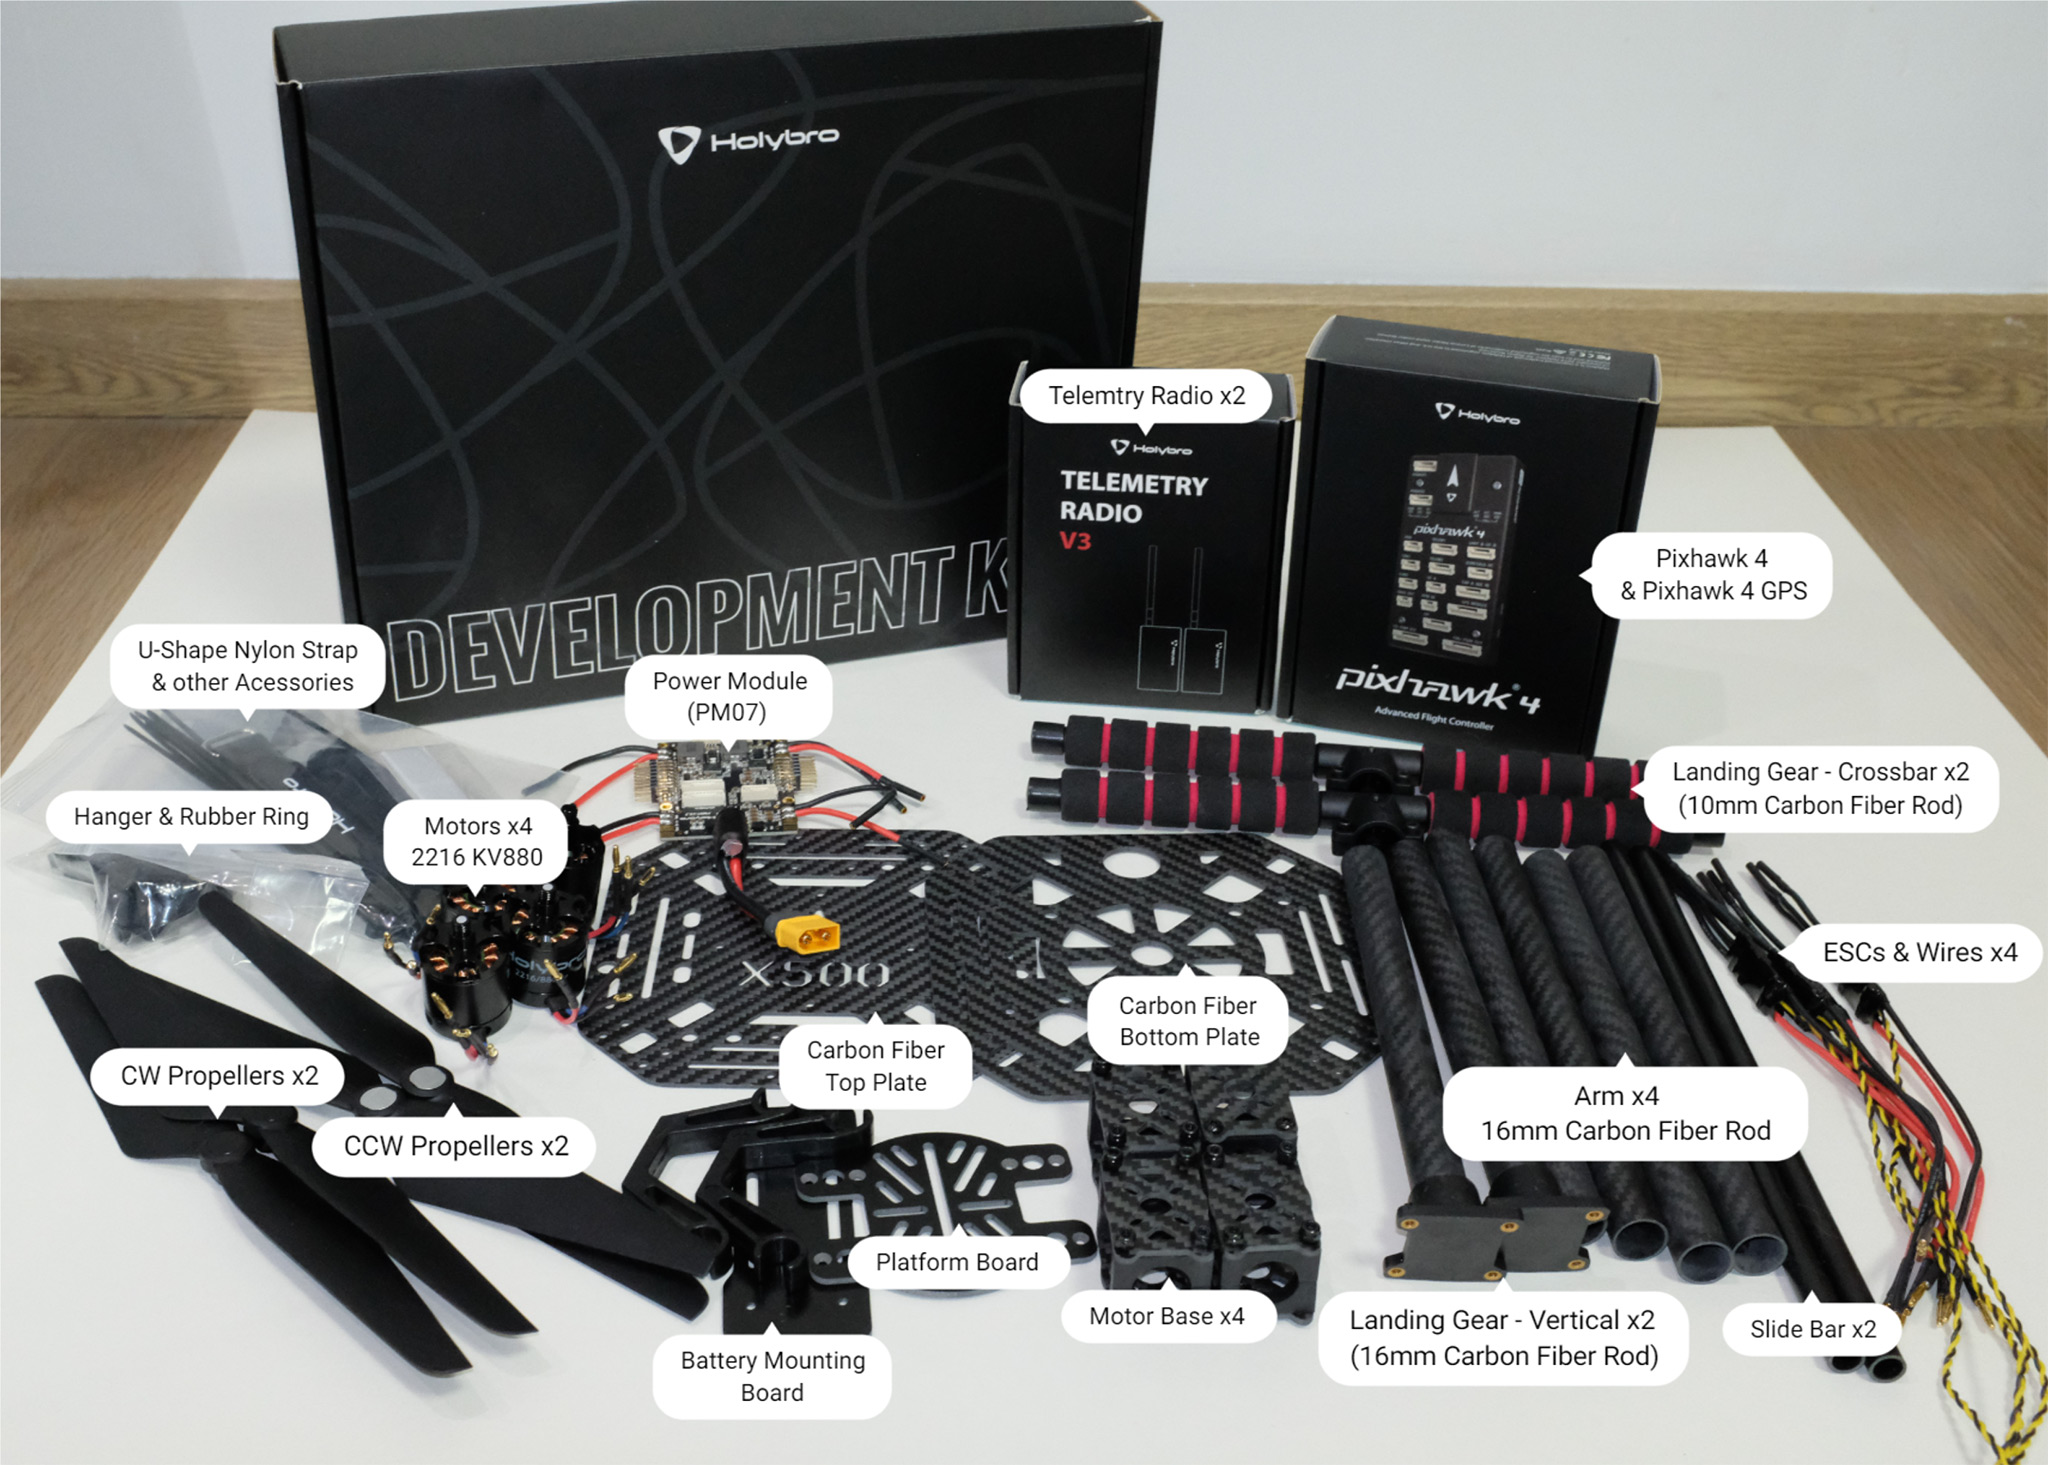
\includegraphics[width=.7\textwidth, keepaspectratio]{img/x500-dev-kit.jpg}
  \caption{Development kit for the Holybro X500.}
  \source{Adapted from \citetitle{px4-guide} \cite{px4-guide}.}
  \label{fig:x500-dev-kit}
\end{figure}


Once the standard parts are assembled, the custom additions can be integrated into the remaining space within the frame. The Raspberry Pi companion computer will be positioned between the autopilot and GPS antenna. This placement facilitates a convenient connection between the autopilot and the Raspberry Pi's I/O pins using short cables, preventing excessive wire clutter within the frame. 

During flight, the Raspberry Pi will be powered by a dedicated external battery, which supplies power through a 2-ampere USB port. This port will be connected to the Raspberry Pi's original power cable, utilizing its USB-C power supply socket. As explained in Section \ref{sec:test-5-rpi}, this power supply is sufficient to operate the connected camera and run the developed software with satisfactory performance. The battery will be positioned beneath the autopilot, as depicted in Figure \ref{fig:full-build}. 


To ensure the camera is securely mounted on the vehicle's frame, the custom-built support system described in Section \ref{subsec:onboard} will be utilized. The camera holder will be attached to the slide bars beneath the main frame, positioning the camera's weight as close to the centre of mass as possible behind the GPS platform. The main battery, responsible for powering the engines and autopilot, and located on the underside of the carbon frame, can be shifted along the forward axis to balance the added weight from the companion computer, its battery and the camera so that the centre of gravity falls approximately in the centre of the vehicle. Figure \ref{fig:camera-holder-closeup} shows the vehicle's underside with the attached camera and the strap for holding the main battery.

\begin{figure}
  \centering
  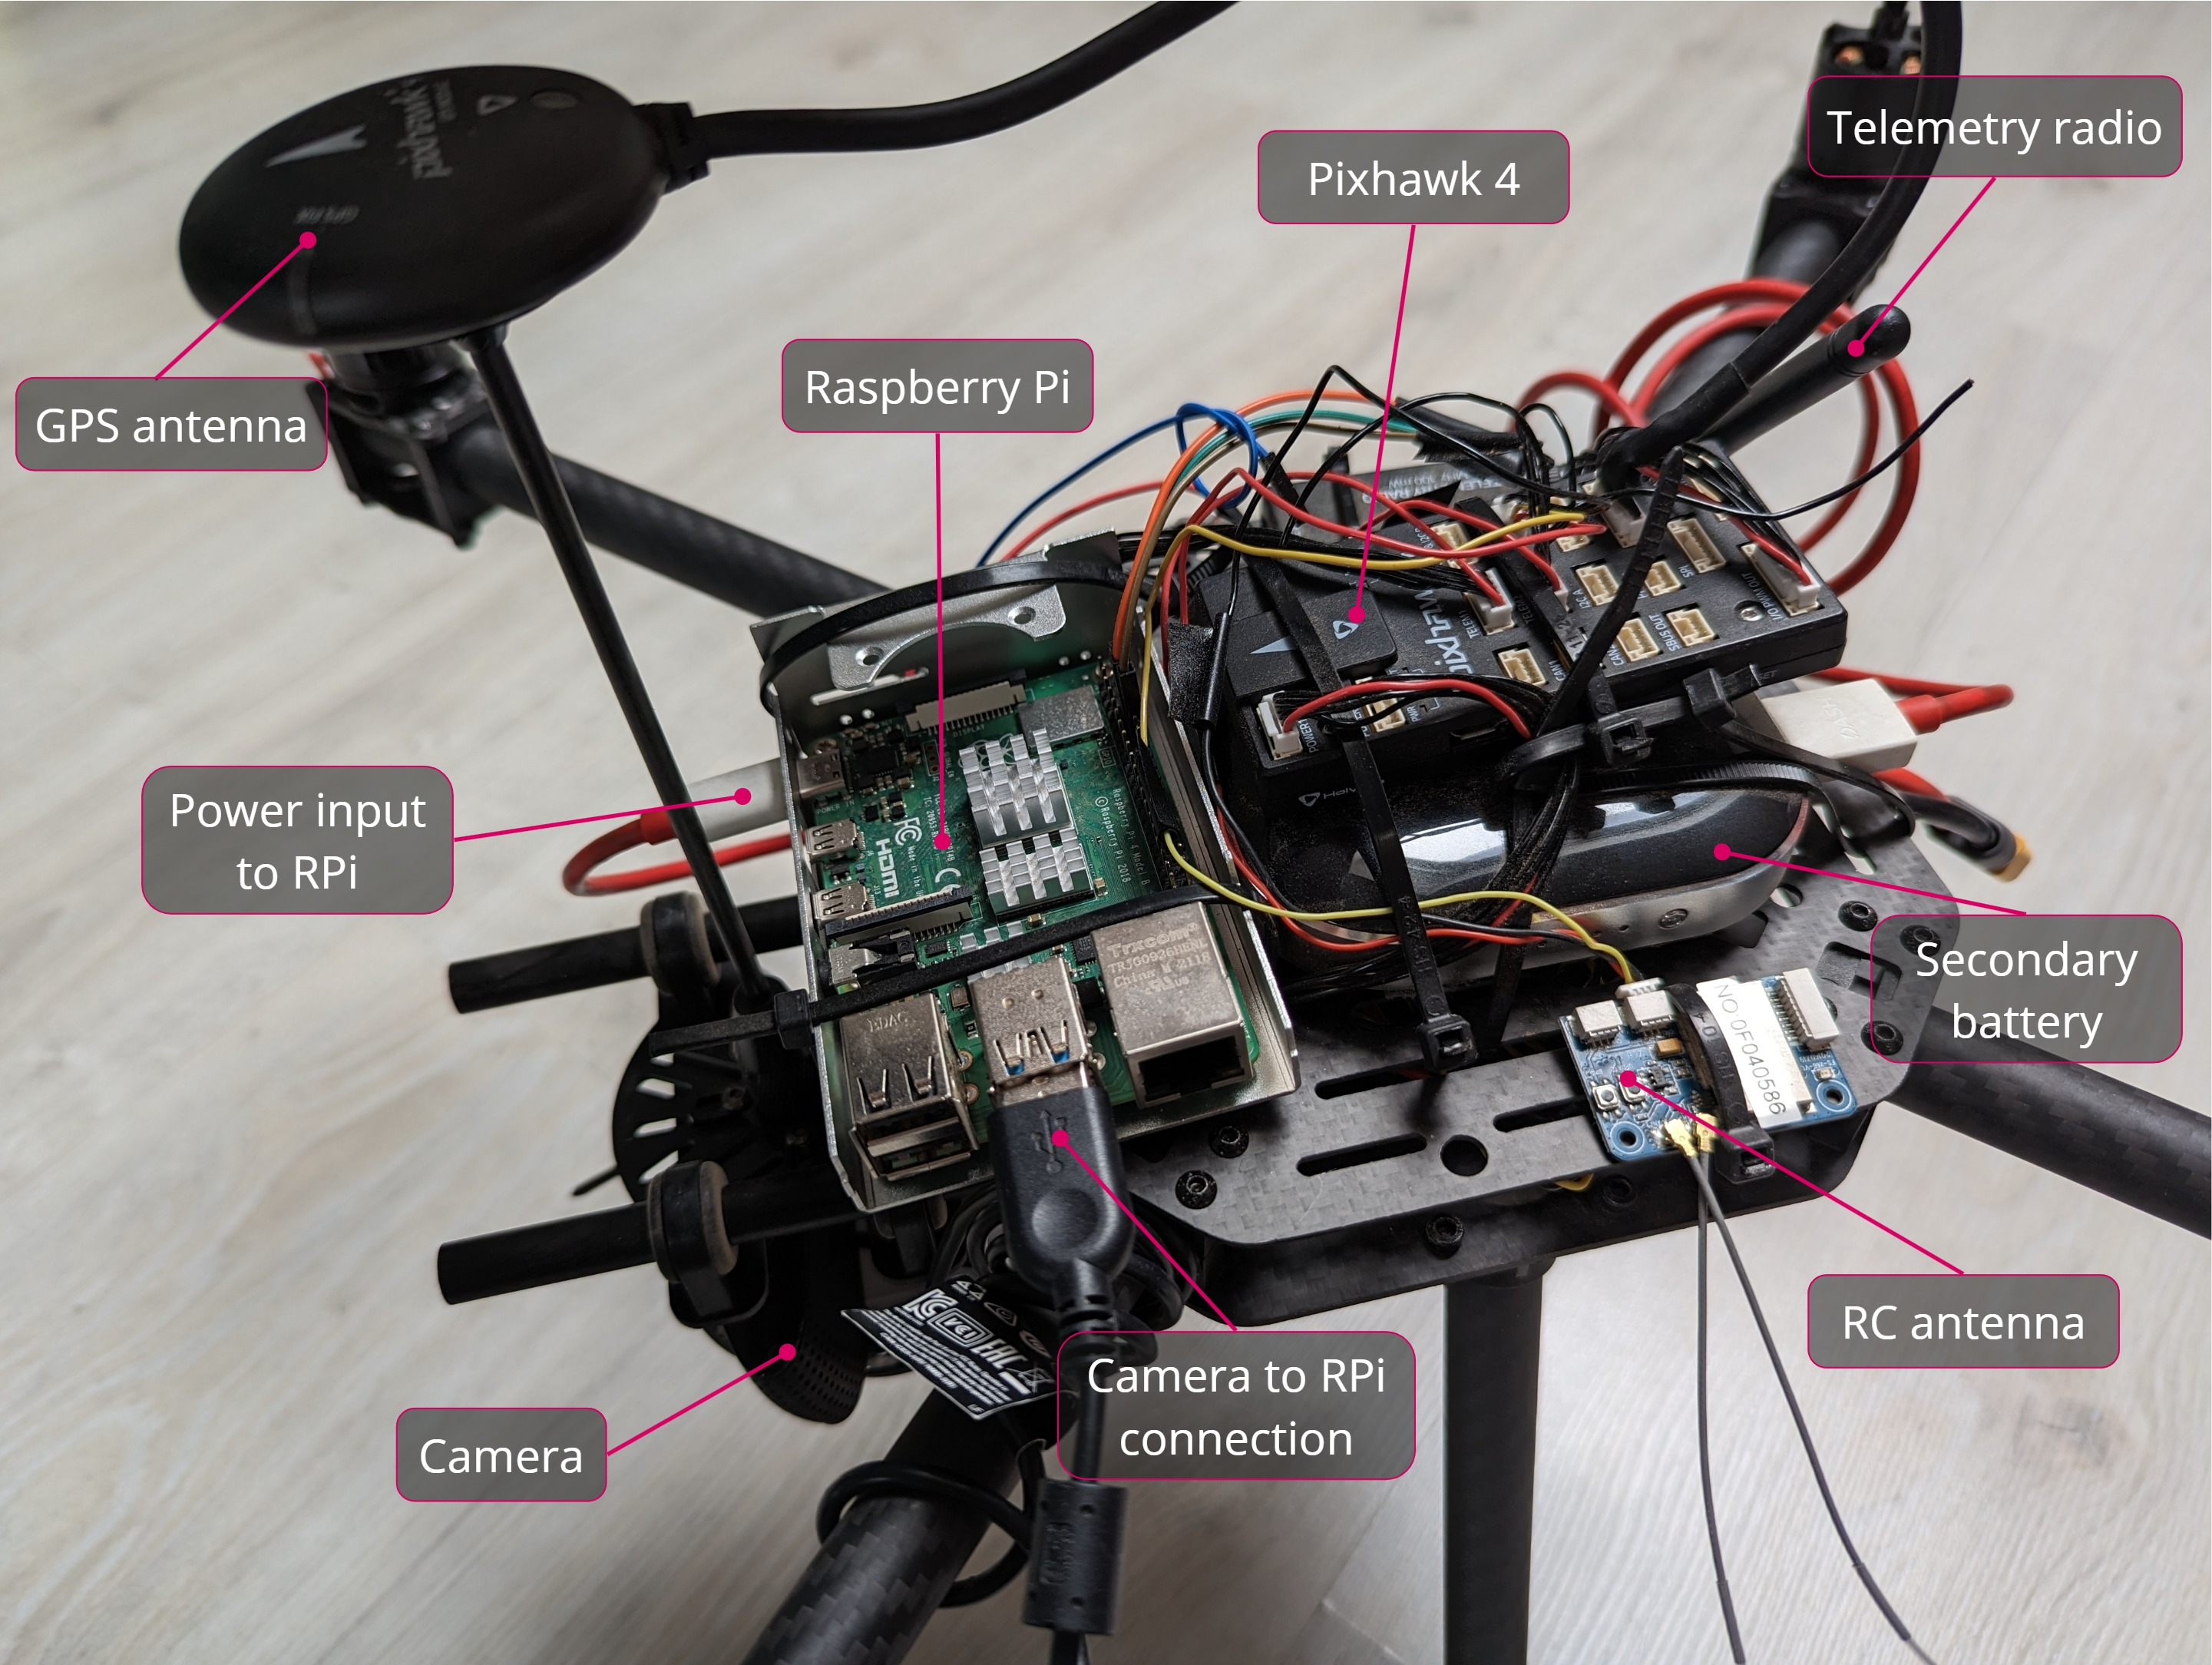
\includegraphics[width=1\textwidth, keepaspectratio]{img/full-build.jpg}
  \caption{Complete build of the quadcopter with the main components highlighted.}\label{fig:full-build}
\end{figure}

\begin{figure}
  \centering
  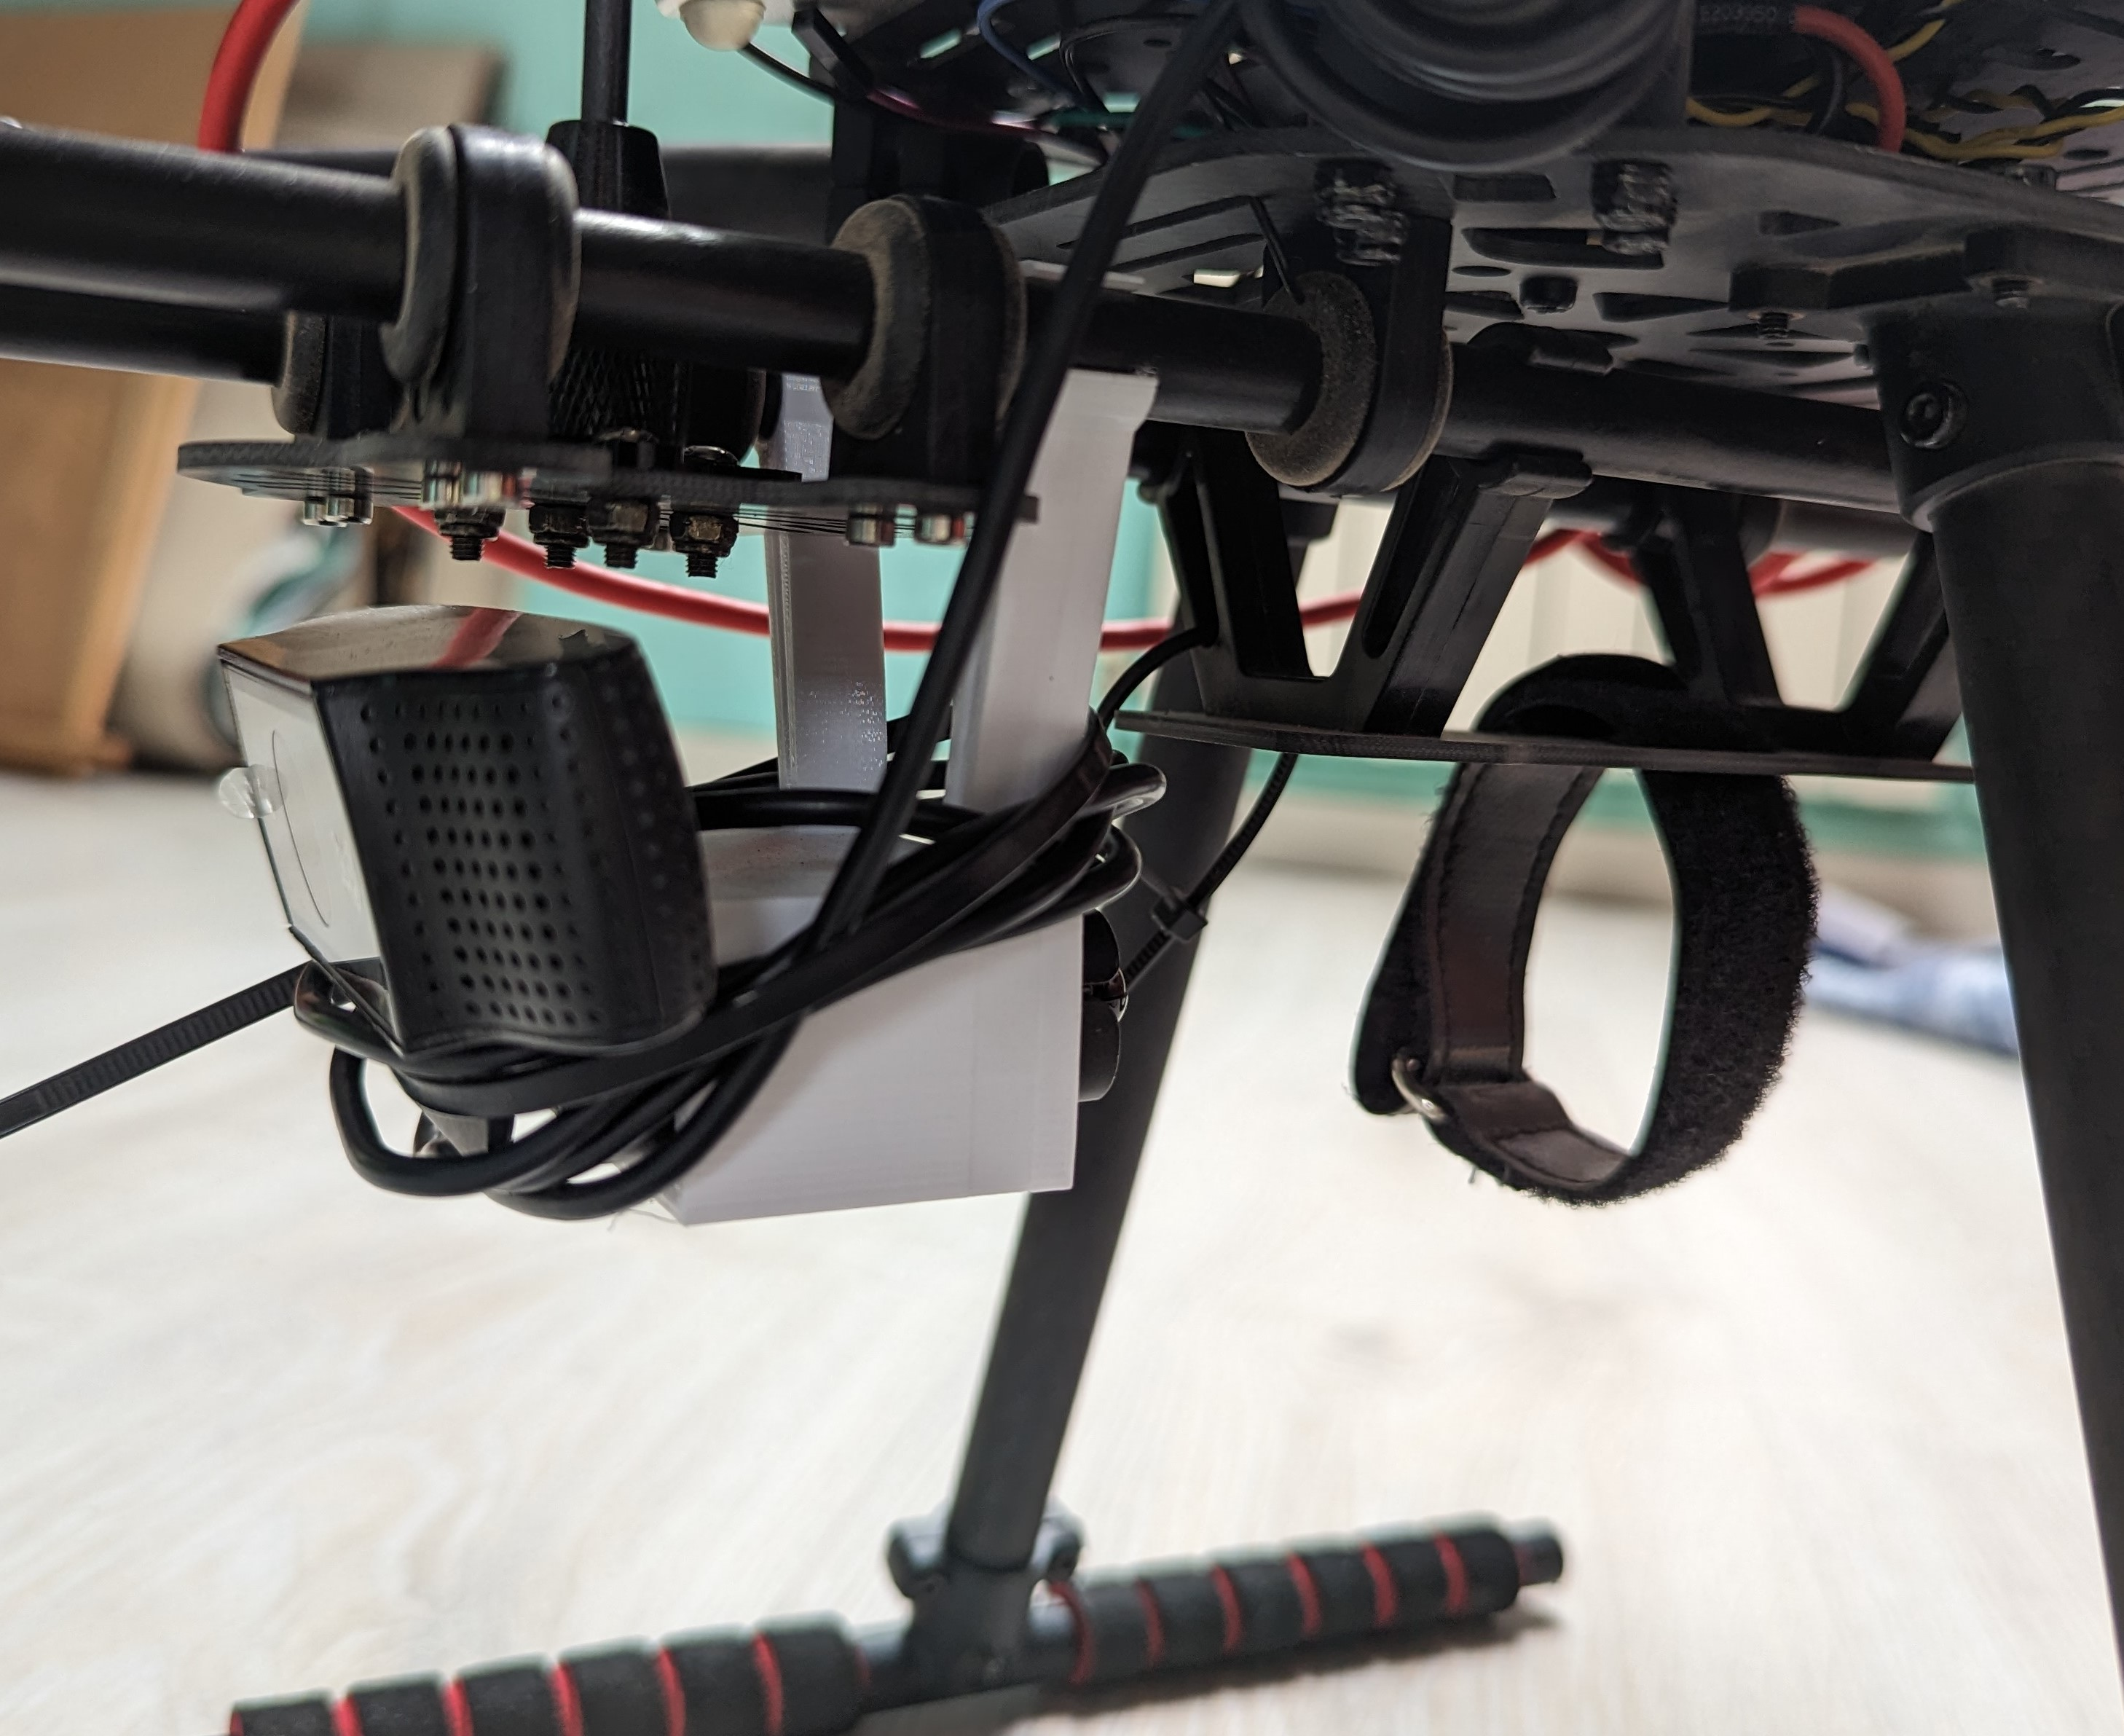
\includegraphics[width=0.7\textwidth, keepaspectratio]{img/underside-2.jpg}
  \caption{Underside of the vehicle, with the supports for holding the main battery and the camera in place.}
  \label{fig:camera-holder-closeup}
\end{figure}


% After the vehicle has been built, there are additional installation and calibration steps that must be carried out before it can fly, also contained in the guide mentioned above.
% Any simulation modes previously activated for testing must be deactivated from the Safety section of the vehicle configuration and the \texttt{MAV\_1\_CONFIG} parameter set to \texttt{TELEM2}, as described in section \ref{subsec:offboard}.
% Then all the different sensors present, both embedded on the flight controller board and attached to the outside frame, need to be calibrated for this particular build.
% The QGroundControl \ref{subsec:qgc} ground station application contains a configuration screen with all the calibration tools needed for the vehicle setup, shown in figure \ref{fig:qgc-config}.
% The vehicle can be configured either by connecting the flight controller directly to the computer via the micro-USB port on its side or through a wireless connection by plugging the companion telemetry radio into the computer running QGroundControl.
Once the vehicle construction is complete, additional installation and calibration steps are necessary before it can be flown. These steps, outlined in the aforementioned guide, include the deactivation of any previously activated simulation modes from the Safety section of the vehicle configuration. Furthermore, the \texttt{MAV_1_CONFIG} parameter must be set to \texttt{TELEM2}, as explained in Section \ref{subsec:offboard}. Calibration of all the onboard and externally attached sensors specific to this build is also required. The QGroundControl ground station application (refer to Section \ref{subsec:qgc}) provides a configuration screen with the necessary calibration tools for vehicle setup, as depicted in Figure \ref{fig:qgc-config}. The vehicle configuration can be performed either by directly connecting the flight controller to a computer via the micro-USB port or wirelessly by connecting the companion telemetry radio to the computer running QGroundControl.


\begin{figure}
  \centering
  \makebox[\textwidth][c]{
  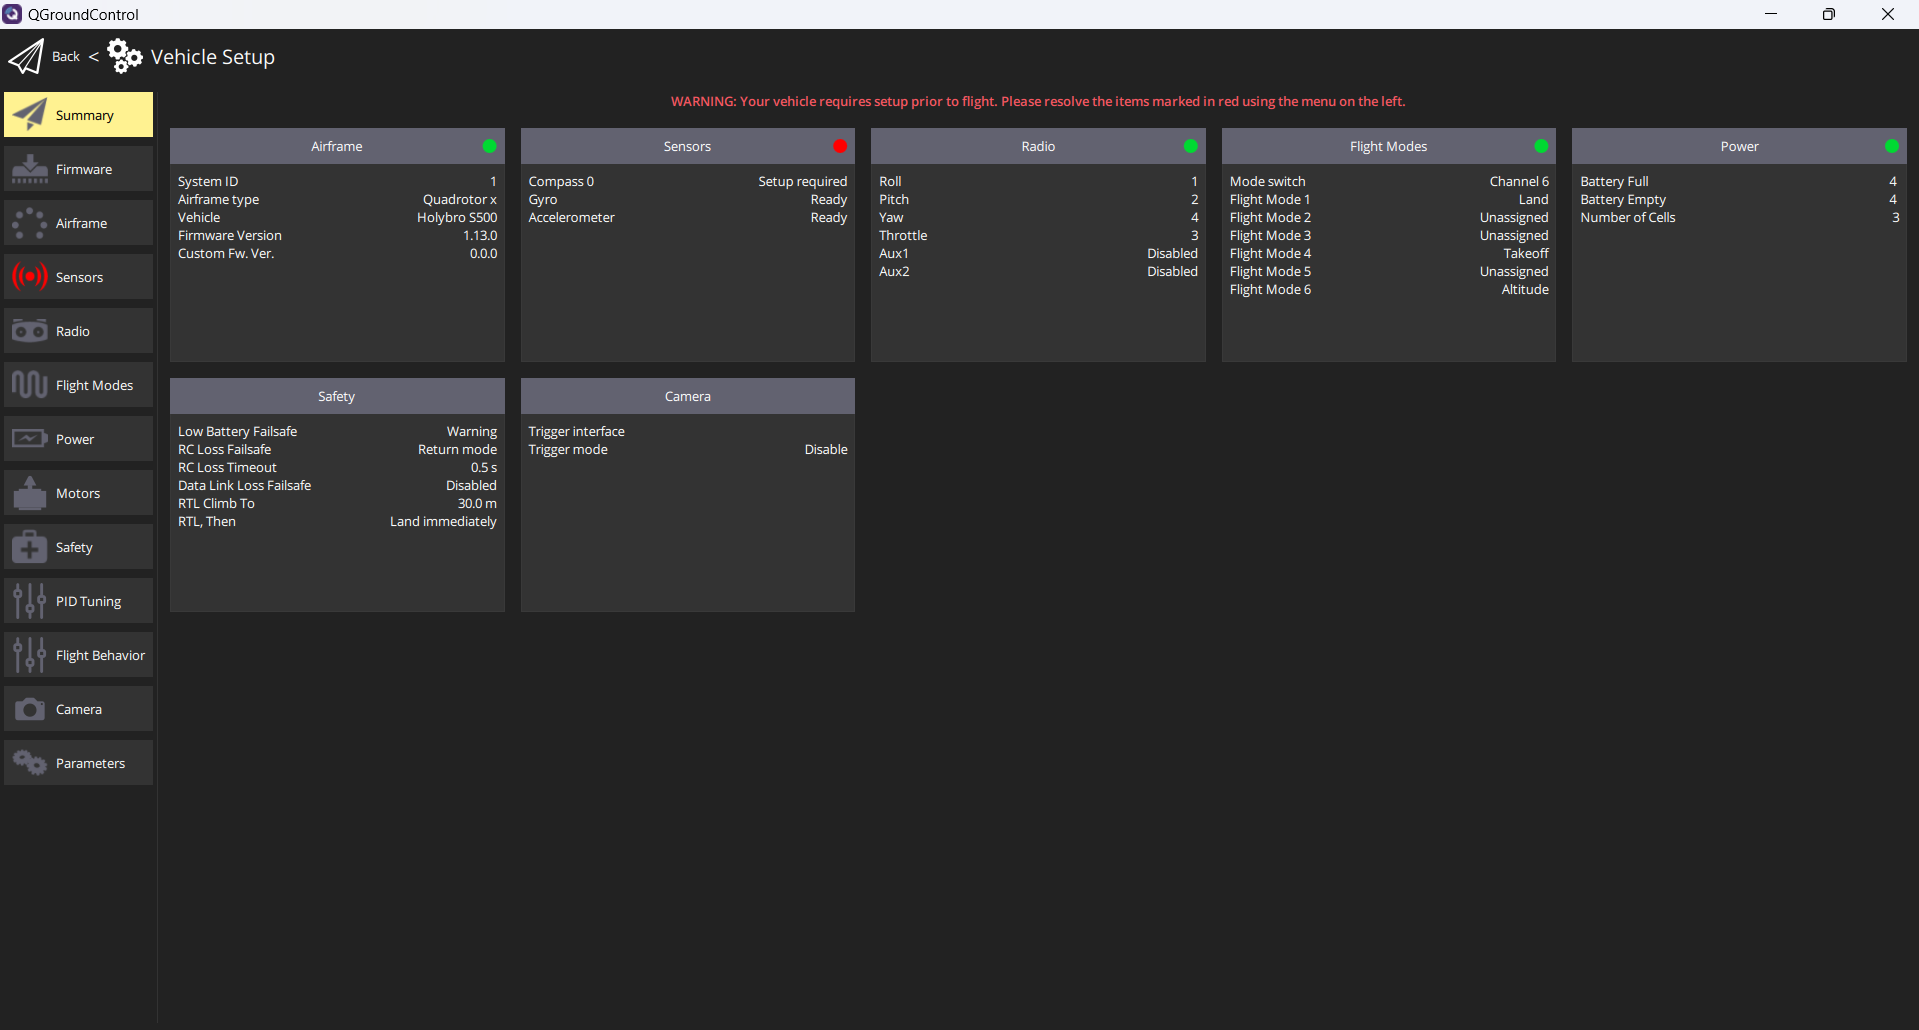
\includegraphics[width=0.5\textwidth, keepaspectratio]{img/qgc-config-1.png}
  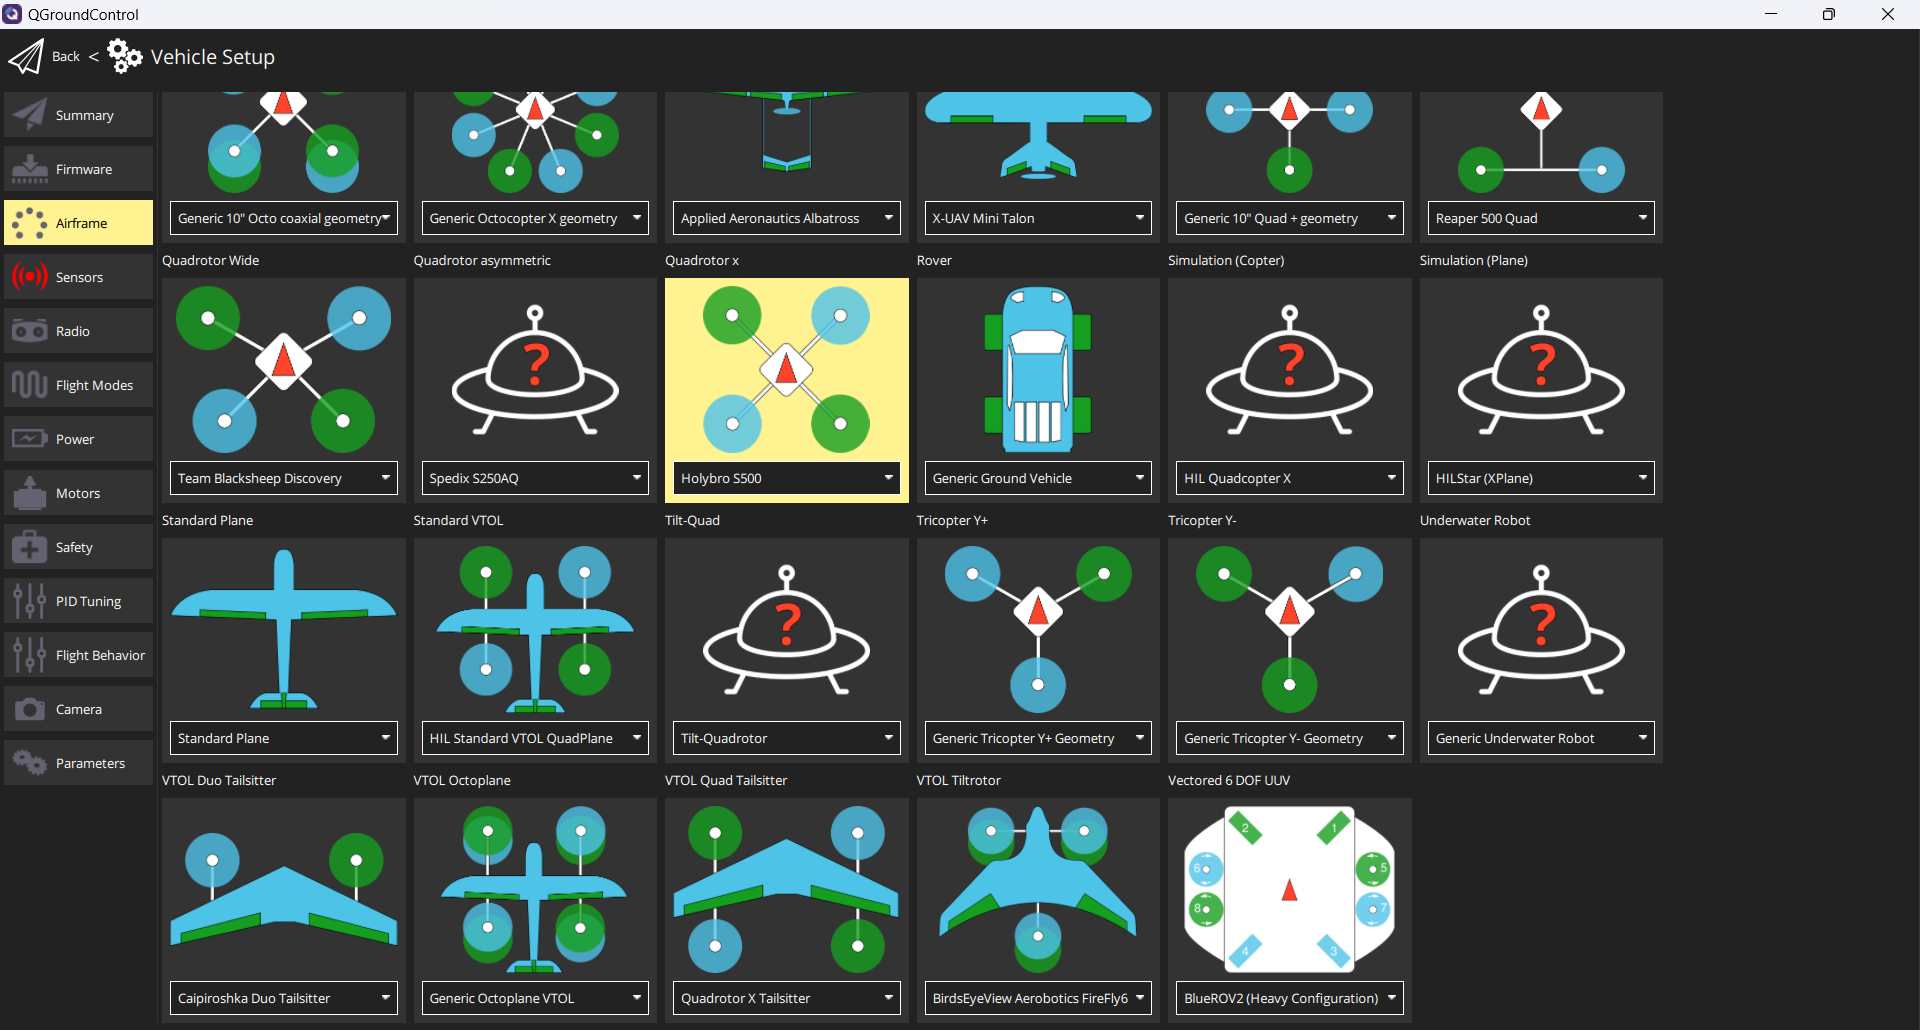
\includegraphics[width=0.5\textwidth, keepaspectratio]{img/qgc-config-3.png}}\\
  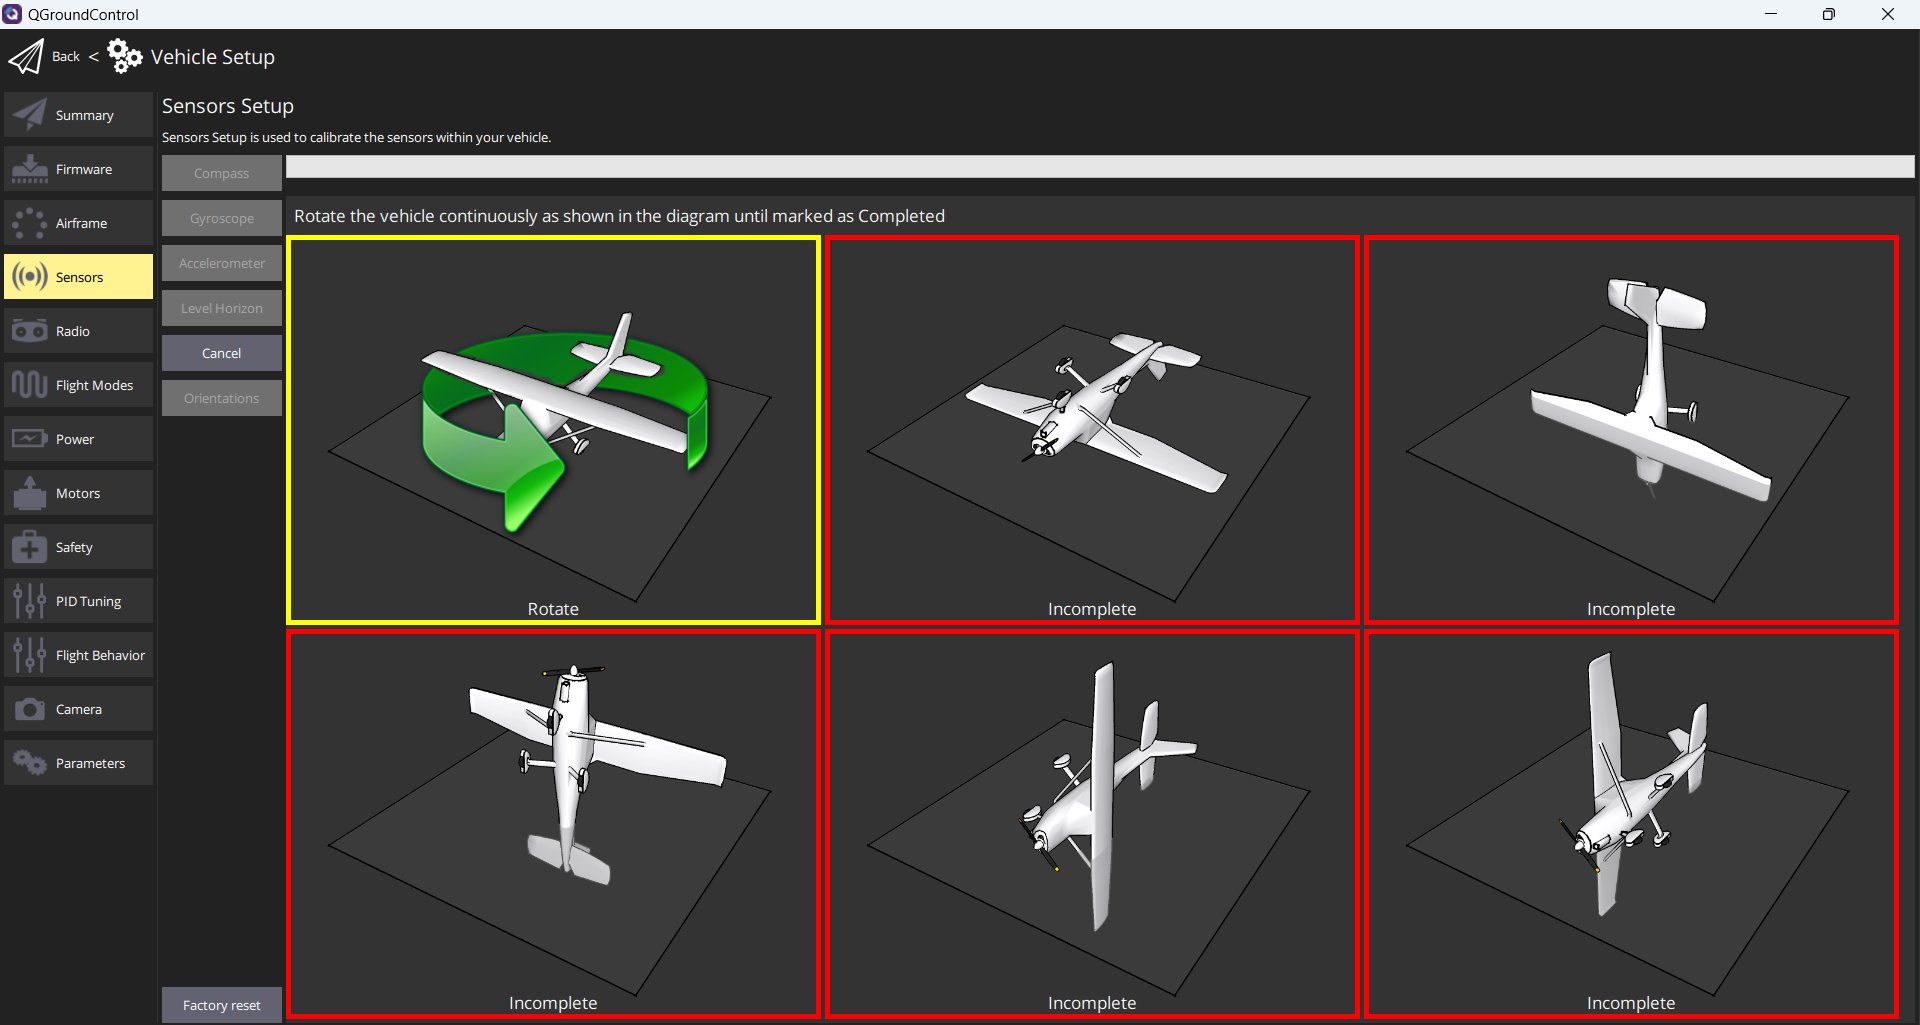
\includegraphics[width=0.5\textwidth, keepaspectratio]{img/qgc-config-2.png}
  \caption{Screenshot from the QGroundControl calibration and setup tools used to configure the vehicle}\label{fig:qgc-config}
\end{figure}


\subsection{Initial tests}
\label{sec:test-8-flight}

% Setup:    flight plan
% Test:     - assisted takeoff, fly with RC
%           - tools/test_camera + record video
% Results:  video of flying, adjust pid set-point

\subsubsection{Baseline flight with factory software}
\label{subsec:fl-test-1}

% Once the vehicle is fully configured, the RC controller and QGroundControl can be used to test assisted takeoff and landing.
% At this point, the drone should be able to maintain stable flight while using autopilot-assisted flight modes like Position Mode, where the roll and pitch sticks control the acceleration over the ground of the vehicle in the forward/backward and left/right directions relative to the heading the vehicle is facing.
% The throttle controls the speed of ascent and descent. 
% With the sticks centred, the vehicle will actively remain locked to a position in 3D space, compensating for wind and other forces.
% This is the safest manual mode to test that the standard autopilot works as expected.
Once the vehicle is fully configured, testing the assisted takeoff and landing can be conducted using the RC controller and QGroundControl. At this stage, the drone should be capable of maintaining stable flight using autopilot-assisted flight modes, such as Position Mode. In Position Mode, the roll and pitch sticks control the vehicle's acceleration over the ground in the forward/backward and left/right directions relative to the vehicle's heading. The throttle stick controls the ascent and descent speed. When the sticks are centered, the vehicle actively maintains its position in 3D space, compensating for wind and external forces. This manual mode serves as a safe means to verify the functionality of the standard autopilot.

% Through QGroundControl it is possible to map the different switches in the RC controller to various autopilot commands.
% For this test, one of the switches with two positions will be mapped to arm/disarm, which controls whether the engines of the quadcopter can start or not. One of the switches with three positions will be mapped to the landing/takeoff/position flight modes, respectively. The main autopilot modes can be tested by switching between the available positions during flight.
% This configuration exhausts all the channels available in the RC controller employed.
% Other flight modes can be set by using the QGroundControl interface directly.
Through QGroundControl, it is possible to map different switches on the RC controller to various autopilot commands. For the test, a two-position switch will be mapped to arm/disarm, controlling the quadcopter's engine startup. A three-position switch will be assigned to the landing/takeoff/position flight modes, respectively. By switching between the available positions during flight, the primary autopilot modes can be tested. It's worth noting that this configuration utilizes all available channels on the RC controller. Additional flight modes can be set directly through the QGroundControl interface.

% To carry out the flight, first, the main battery is connected to the socket in the power module.
% This starts up the autopilot, the GPS antenna, the telemetry radio, and the RC receiver.
% Afterwards, QGroundControl can be started on a computer connected to the second telemetry radio via USB.
% If everything has worked correctly, the ground station application will automatically connect to the vehicle and situate its position on a satellite map.
% Turning on the RC controller will likewise make it connect to the vehicle, as long as it has been paired correctly, as indicated in the guide linked in the first step of the build process.
% Once all the wireless connections have been established, the drone can take off by first switching to the armed state and then switching to the takeoff flight mode.
% While the drone is in the air, switching to the position flight mode will allow direct control through the joysticks in the controller.
To initiate the flight, the main battery is connected to the power module socket. This action powers up the autopilot, GPS antenna, telemetry radio, and RC receiver. Subsequently, QGroundControl is launched on a computer connected to the second telemetry radio via USB. If all connections have been established correctly, the ground station application will automatically connect to the vehicle and display its position on a satellite map. Similarly, turning on the RC controller, provided it has been correctly paired as outlined in the guide from the initial build process, establishes the connection with the vehicle. Once all wireless connections are established, the drone can take off by switching to the armed state, followed by selecting the takeoff flight mode. While the drone is airborne, switching to the position flight mode enables direct control through the joysticks on the controller.


\subsubsection{Offboard computer flight with test tool}
\label{subsec:fl-test-2}

% The second test flight will aim to ensure that the custom software can send takeoff and landing commands through a wireless MAVlink channel from the offboard computer (using the telemetry radio through the developed test tool).
% For this flight, the QGroundControl application cannot be connected to the vehicle since the DroneVisionControl application will block the telemetry radio channel.
% The RC controller will therefore be used as a backup in case anything goes wrong with the software.
% At any moment, the controller can switch flight mode and override the input generated from the DroneVisionControl application, recovering manual control.
The second test flight aims to verify that the custom software can wirelessly transmit takeoff and landing commands from the offboard computer using a MAVlink channel (utilizing the telemetry radio through the developed test tool). During this flight, it is important to note that the QGroundControl application cannot be connected to the vehicle as it will interfere with the telemetry radio channel used by the DroneVisionControl application. Consequently, the RC controller will serve as a backup in case of any issues with the software. The controller can be used to switch flight modes and override inputs from the DroneVisionControl application, providing manual control if necessary.


% Since the DroneVisionControl application can now easily arm the vehicle on its own while sending a takeoff command,
% the two-way switch of the controller will be mapped for all the tests from now on to the command to kill the power to the engines.
% This command could be helpful in edge cases to protect the vehicle or the surrounding area if the autopilot were to destabilize during takeoff and landing or completely lose control over the vehicle.
% Now, once the main battery is connected again to the power module, the test tool is run with the following command for a Windows or a Linux machine, respectively:
% \begin{minted}[breaklines, fontsize=\footnotesize, baselinestretch=1]{bash}
% dronevisioncontrol tools test-camera -r COM<X>:57600
% \end{minted}
% or
% \begin{minted}[breaklines, fontsize=\footnotesize, baselinestretch=1]{bash}
% dronevisioncontrol tools test-camera -r /dev/ttyUSB0:57600
% \end{minted}
To ensure flexibility and safety during the tests, the two-way switch on the controller will be mapped to the command to cut off power to the engines. This command can be valuable in exceptional situations where it is necessary to protect the vehicle or the surrounding area, such as during destabilization or complete loss of control by the autopilot during takeoff, landing, or flight.

To initiate the test, reconnect the main battery to the power module. Then, execute the following command on the offboard computer, depending on whether it is a Windows or Linux machine:

For Windows: dronevisioncontrol tools test-camera -r COM<X>:57600
For Linux: dronevisioncontrol tools test-camera -r /dev/ttyUSB0:57600

% After successfully connecting to the vehicle, the T and L keys in the computer keyboard can be used for takeoff and landing, respectively. The O key can be used to set the autopilot in offboard flight mode to enable it to receive velocity commands.
% Afterwards, the WASD keys can be used to control the forward and sideways velocity of the vehicle and the QE keys to control its yaw velocity.
% Figure \ref{fig:flight-test-cam-offboard} displays the output on the computer's terminal window, where the connection process and the sent velocity commands are shown, and the output on the camera from the offboard computer.
% A video of the entire process can be found \href{https://l-gonz.github.io/tfg-giaa-dronecontrol/videos/flight-test-offboard}{here}\footnote{\url{https://l-gonz.github.io/tfg-giaa-dronecontrol/videos/flight-test-offboard}}.
After successfully establishing the connection with the vehicle, the computer keyboard can be used to control the flight. Pressing the T key triggers takeoff, while the L key initiates the landing process. The O key sets the autopilot to offboard flight mode, enabling it to receive velocity commands. Subsequently, the WASD keys control the forward and sideways velocity of the vehicle, and the QE keys adjust its yaw velocity.

Figure \ref{fig:flight-test-cam-offboard} illustrates the output displayed in the computer's terminal window, showcasing the connection process, the sent velocity commands, and the camera output from the offboard computer. Additionally, a video capturing the entire process can be accessed using the provided link.

\begin{figure}
  \centering
  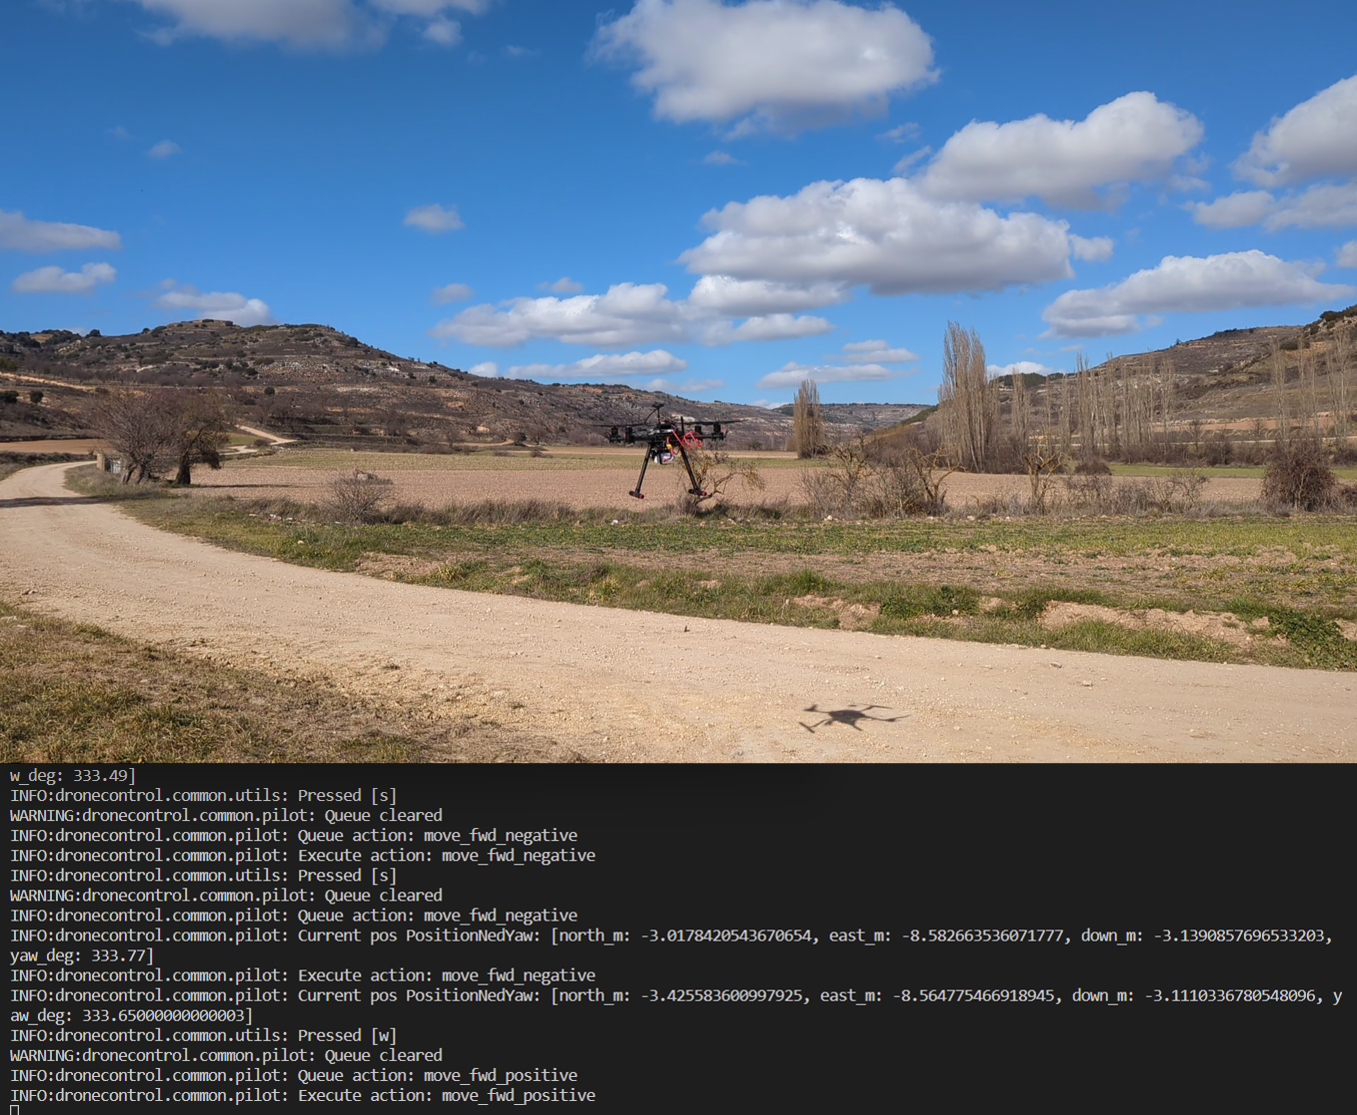
\includegraphics[width=\textwidth, keepaspectratio]{img/video-field-test-offboard.png}
  \caption{Terminal output from the \texttt{test-camera} tool running on an offboard computer and image of the drone flying in response}
  \label{fig:flight-test-cam-offboard}
\end{figure}

\subsubsection{Onboard computer flight with test tool}
\label{subsec:fl-test-3}

% The third and last test flight in this section will ensure that the custom software can send takeoff and landing commands through a cabled MAVlink channel from the onboard computer,
% as well as ensuring that the onboard camera can obtain a good image of the field of view of the vehicle during flight.
% For that, the same tool will be used as in the last test, 
% but in this instance, it will be run on the Raspberry Pi, and the connection will be established through the wired serial link between this onboard computer and the Pixhawk autopilot board.
% Since the camera connected to the computer sending commands is now looking down on the pilot, it is possible to activate pose detection on the test images received from this onboard camera.
The third and final test flight in this section aims to confirm that the custom software can send takeoff and landing commands through a cabled MAVlink channel from the onboard computer. Additionally, it ensures that the onboard camera can capture a clear image of the vehicle's field of view during flight.

To perform this test, the same tool used in the previous test will be executed on the Raspberry Pi, utilizing the wired serial link between the onboard computer and the Pixhawk autopilot board. As the camera connected to the computer is positioned to look down on the pilot, pose detection can be activated on the received test images from this onboard camera.

% To start the flight test, the main and secondary batteries need to be attached, respectively, to the power module and to the Raspberry Pi.
% After the onboard computer has started, the easiest way to control it is with a remote desktop connection through WiFi, as explained in section \ref{sec:devenv}.
% By this connection, a terminal window can be opened on the desktop, and the following command run:
To initiate the flight test, attach the main battery to the power module and the secondary battery to the Raspberry Pi. Once the onboard computer has started, establish a remote desktop connection via WiFi, following the instructions provided in section \ref{sec:devenv}. Through this connection, open a terminal window on the desktop and execute the following command:
\begin{minted}[breaklines, fontsize=\footnotesize, baselinestretch=1]{bash}
dronevisioncontrol tools test-camera -r /dev/serial0:921600 -p
\end{minted}


% As opposed to the flight using the telemetry radio, in this test, the serial connection runs at a baudrate of 921600, which matches the configured baudrate on the \texttt{TELEM2} port of the Pixhawk board.
% The "-p" option enables pose detection in the output images.
% A video of the entire process can be found \href{https://l-gonz.github.io/tfg-giaa-dronecontrol/videos/flight-test-onboard}{here}\footnote{\url{https://l-gonz.github.io/tfg-giaa-dronecontrol/videos/flight-test-onboard}} and an image extracted form it can be seen in figure \ref{fig:flight-test-cam-onboard}.
Unlike the telemetry radio flight, this test employs a serial connection running at a baud rate of 921600, matching the configured baud rate on the \texttt{TELEM2} port of the Pixhawk board. The "-p" option enables pose detection in the output images.

A video documenting the entire process can be accessed at the following link: Flight Test Onboard Video. Additionally, an image extracted from the video can be seen in Figure \ref{fig:flight-test-cam-onboard}.


\begin{figure}
  \centering
  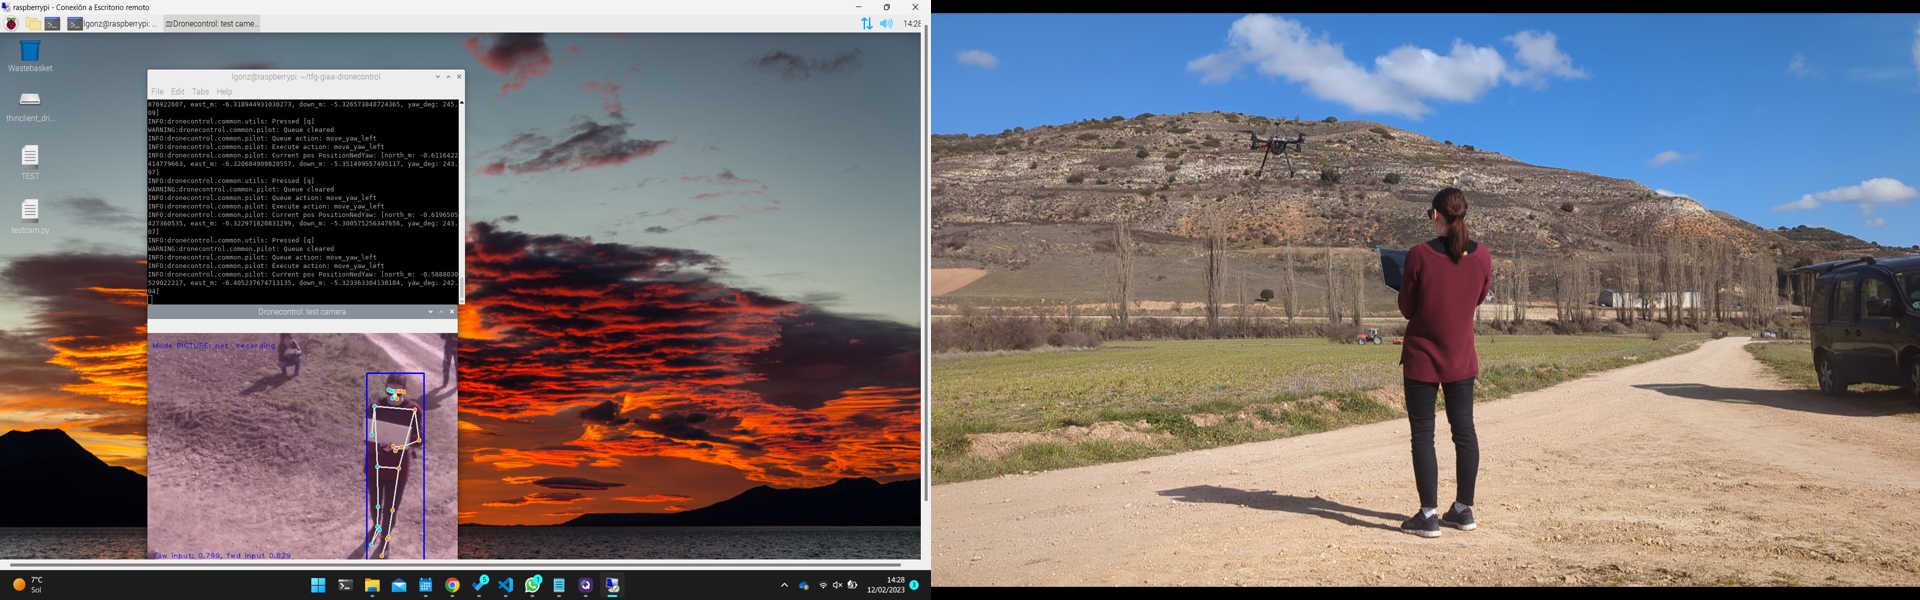
\includegraphics[width=\textwidth, keepaspectratio]{img/video-field-test-onboard.png}
  \caption{Pose detection algorithm running on images taken during flight}
  \label{fig:flight-test-cam-onboard}
\end{figure}


\subsection{Hand gesture control}
\label{subsec:fl-test-4}

% During basic flight tests, all the connections and individual parts of the software were validated in actual flight.
% Now, it is time to integrate the piloting system with the image recognition results to test the developed vision-based control solutions.
% The first solution to be used in flight will be the hand-gesture guidance system, which runs on an offboard computer with more available processing resources and no dependence on battery-supplied power to work.
% The setup will be identical to the second test flight (\ref{subsec:fl-test-2}) with the telemetry radio as the serial link and the onboard companion computer turned off.
% Once the autopilot board is powered up, the control solution can be started with the following command:
% \begin{minted}[breaklines, fontsize=\footnotesize, baselinestretch=1]{bash}
% dronevisioncontrol hand -s <device>:57600
% \end{minted}
% where <device> is the COM port or TTY device the telemetry radio is attached to, depending on the platform.
During the basic flight tests, all the connections and individual components of the software were validated in actual flight scenarios. Now, the focus shifts to integrating the piloting system with the results of image recognition to test the developed vision-based control solutions.

The first solution to be tested in flight is the hand-gesture guidance system, which runs on an offboard computer with ample processing resources and doesn't rely on battery power. The setup for this test will be the same as the second test flight described in section \ref{subsec:fl-test-2}, utilizing the telemetry radio as the serial link and turning off the onboard companion computer. Once the autopilot board is powered up, initiate the control solution by executing the following command:
dronevisioncontrol hand -s <device>:57600
Replace <device> with the appropriate COM port or TTY device to which the telemetry radio is connected, depending on the platform.


% After the pilot connects, the image from the computer's webcam will appear on the screen with an outline over any detected hand.
% An open palm should be shown to the camera to start controlling the vehicle.
% Then, a closed fist will make the drone take off, and pointing up with the index finger will start the offboard flight mode.
% Afterwards, moving the index finger right or left will make the vehicle mirror the movement, 
% and moving the thumb right or left will make the vehicle move forward and backwards, respectively.
% At any point during the test, an open hand will make the drone hover at its current place, as will losing sight of the controlling hand.
Once the pilot connection is established, the image from the computer's webcam will be displayed on the screen with an outline highlighting any detected hand. To begin controlling the vehicle, show an open palm to the camera. Closing the hand into a fist will initiate takeoff, and pointing up with the index finger will activate the offboard flight mode. Moving the index finger right or left will cause the vehicle to mirror the movement, while moving the thumb right or left will make the vehicle move forward and backward, respectively. At any point during the test, displaying an open hand will cause the drone to hover in its current position. Losing sight of the controlling hand will also trigger this hovering behavior.


% A video of the entire process can be found \href{https://l-gonz.github.io/tfg-giaa-dronecontrol/videos/flight-test-hand}{here}\footnote{\url{https://l-gonz.github.io/tfg-giaa-dronecontrol/videos/flight-test-hand}} and an image extracted form it can be seen in figure \ref{fig:flight-test-hand}.
A video showcasing the entire process can be accessed at the following link: Flight Test Hand Video. Additionally, an image extracted from the video can be seen in Figure \ref{fig:flight-test-hand}.

\begin{figure}
  \centering
  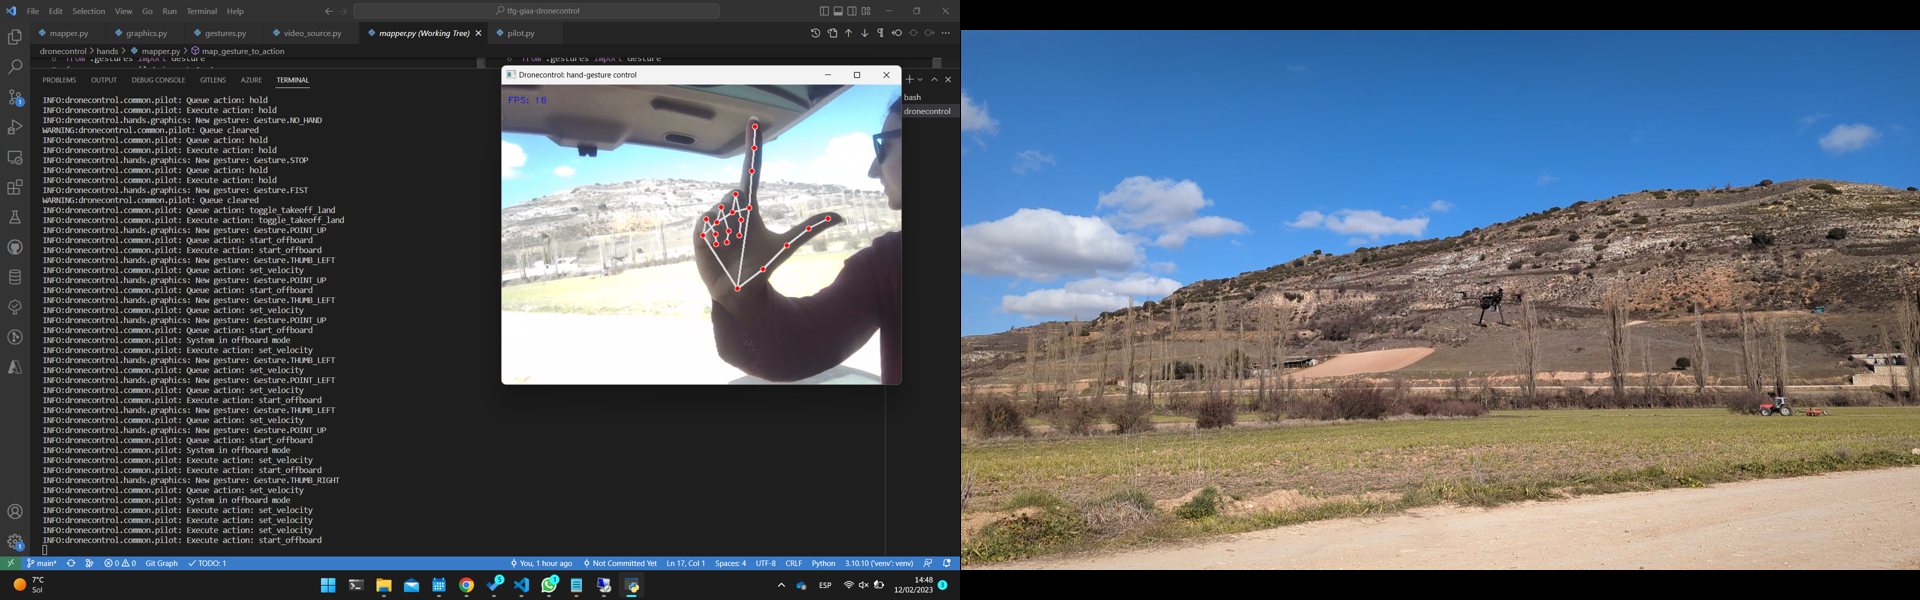
\includegraphics[width=\textwidth, keepaspectratio]{img/video-field-test-hand.png}
  \caption{Image taken during flight controlled by the hand-gesture solution. The vehicle is moving forward.}
  \label{fig:flight-test-hand}
\end{figure}

\subsection{Target detecting, tracking and following}
\label{subsec:fl-test-5}


% Finally, it only remains to test the follow control solution.
% In this section, the companion computer will be running the follow program, and it will be validated whether it can keep track of and follow a moving target during a non-simulated flight.
% The setup will be identical to the third test in section \ref{subsec:fl-test-3}, without needing a wireless telemetry connection.
% The telemetry radio is, therefore, free to be used, for example, to track the vehicle's path through the QGroundControl application on a secondary, offboard computer.
% The control application will be started with the following command:
% \begin{minted}[breaklines, fontsize=\footnotesize, baselinestretch=1]{bash}
% dronevisioncontrol follow -s /dev/serial0:921600
% \end{minted}
% This \href{https://l-gonz.github.io/tfg-giaa-dronecontrol/videos/flight-test-follow}{video}\footnote{\url{https://l-gonz.github.io/tfg-giaa-dronecontrol/videos/flight-test-follow}} shows the process of getting the vehicle to takeoff (T key), activating offboard flight mode (O key), and starting movement tracking of the detected figure.
% Figure \ref{fig:flight-test-follow} shows an image extracted from this video.
To test the follow control solution, the companion computer will run the follow program, aiming to track and follow a moving target during an actual non-simulated flight. The setup for this test will be the same as the third test flight described in section \ref{subsec:fl-test-3}, without the need for a wireless telemetry connection. The telemetry radio can be utilized, for example, to track the vehicle's path using the QGroundControl application on a secondary offboard computer. Initiate the control application by executing the following command:
dronevisioncontrol follow -s /dev/serial0:921600
This video here showcases the process of the vehicle taking off (T key), activating offboard flight mode (O key), and initiating the tracking of a detected figure. Additionally, Figure \ref{fig:flight-test-follow} presents an image extracted from this video.


\begin{figure}
  \centering
  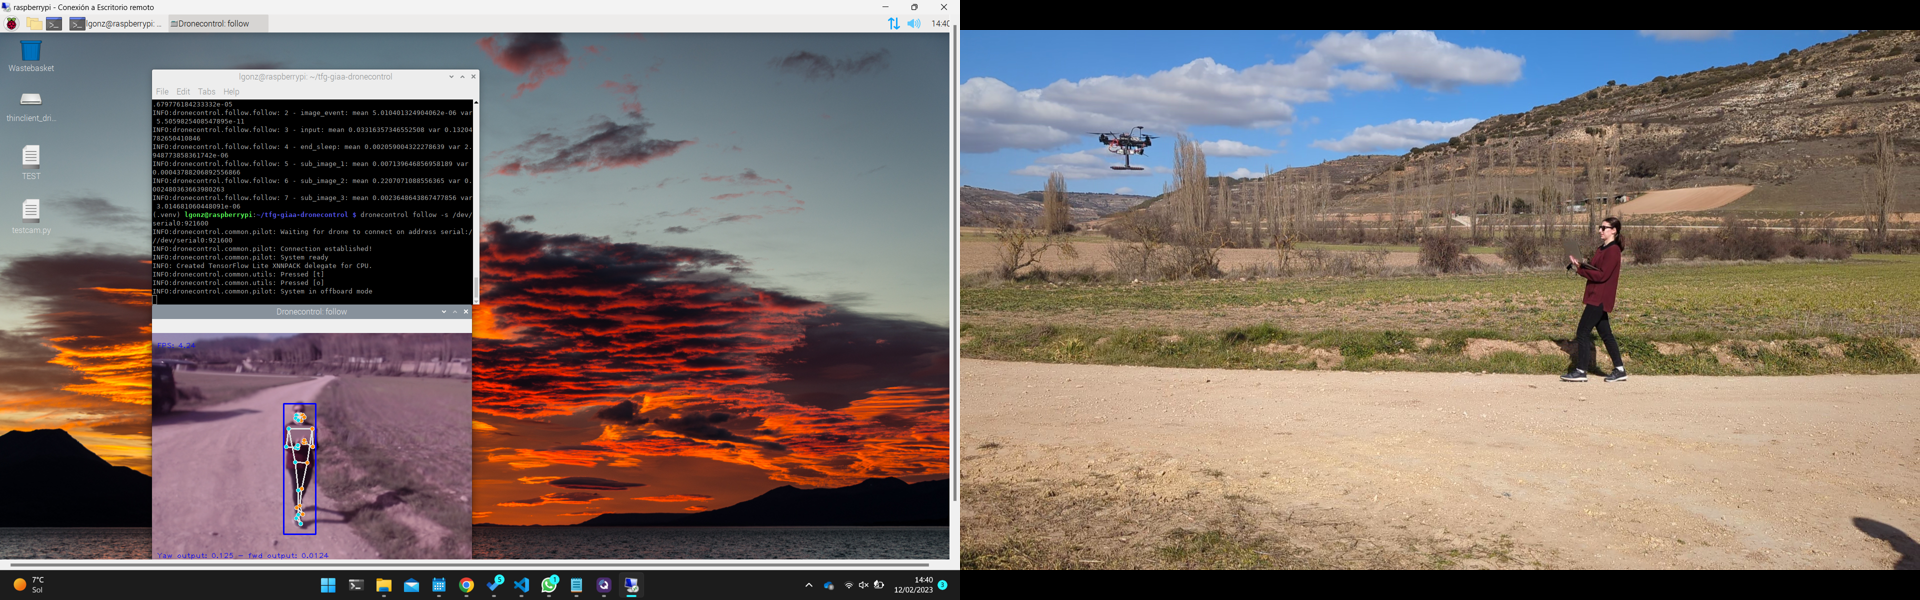
\includegraphics[width=\textwidth, keepaspectratio]{img/video-field-test-follow.png}
  \caption{Terminal and image output of the DroneVisionControl follow solution running on the Raspberry Pi}
  \label{fig:flight-test-follow}
\end{figure}

% The maximum frames per second managed by the program running on the Pi is around 6 FPS when the follow mechanism is engaged and around 8 FPS if it is disabled by switching out of offboard flight mode.
% In practice, this means that the person being tracked by the drone has to move quite slowly for the camera not to lose sight of them before the autopilot can send the command to the vehicle to move to the previously detected position.
% However, for a proof-of-concept scenario, this is an acceptable performance.
During the flight test, the program running on the Raspberry Pi achieves a maximum frame rate of around 6 FPS when the follow mechanism is active, and approximately 8 FPS when it is disabled by switching out of offboard flight mode. In practical terms, this means that the person being tracked by the drone needs to move relatively slowly to ensure that the camera does not lose sight of them before the autopilot can send the command to the vehicle to move to the previously detected position. However, for a proof-of-concept scenario, this performance is acceptable.

% At the end of the program run, the average loop time and average runtime for each of the tasks in the main loop are shown in the terminal.
% From the measures obtained for the test flight carried out, the average frame rate calculates to be 3.58 FPS.
% If these measurements are compared to those analyzed in section \ref{subsec:performance}, as shown in figure \ref{fig:flight-performance}, particularly to the test configuration most closely resembling actual flight with the autopilot board running on HITL mode and the companion computer powered by the secondary battery, it is possible to appreciate how close this configuration matches the behaviour during actual flight and therefore validating it as an appropriate environment to test the performance of this type of algorithms.
At the end of the program execution, the average loop time and average runtime for each task in the main loop will be displayed in the terminal. Based on the measurements obtained during the test flight, the average frame rate calculates to be 3.58 FPS. Comparing these measurements with those analyzed in section \ref{subsec:performance}, particularly with the test configuration that closely resembles actual flight with the autopilot board running on HITL mode and the companion computer powered by the secondary battery (as shown in Figure \ref{fig:flight-performance}), it is evident that this configuration closely matches the behavior during actual flight. This validates it as a suitable environment for testing the performance of such algorithms.

Overall, this test flight verifies the effectiveness of the follow control solution and its ability to track and follow a moving target during a real flight scenario.


\begin{figure}
  \centering
  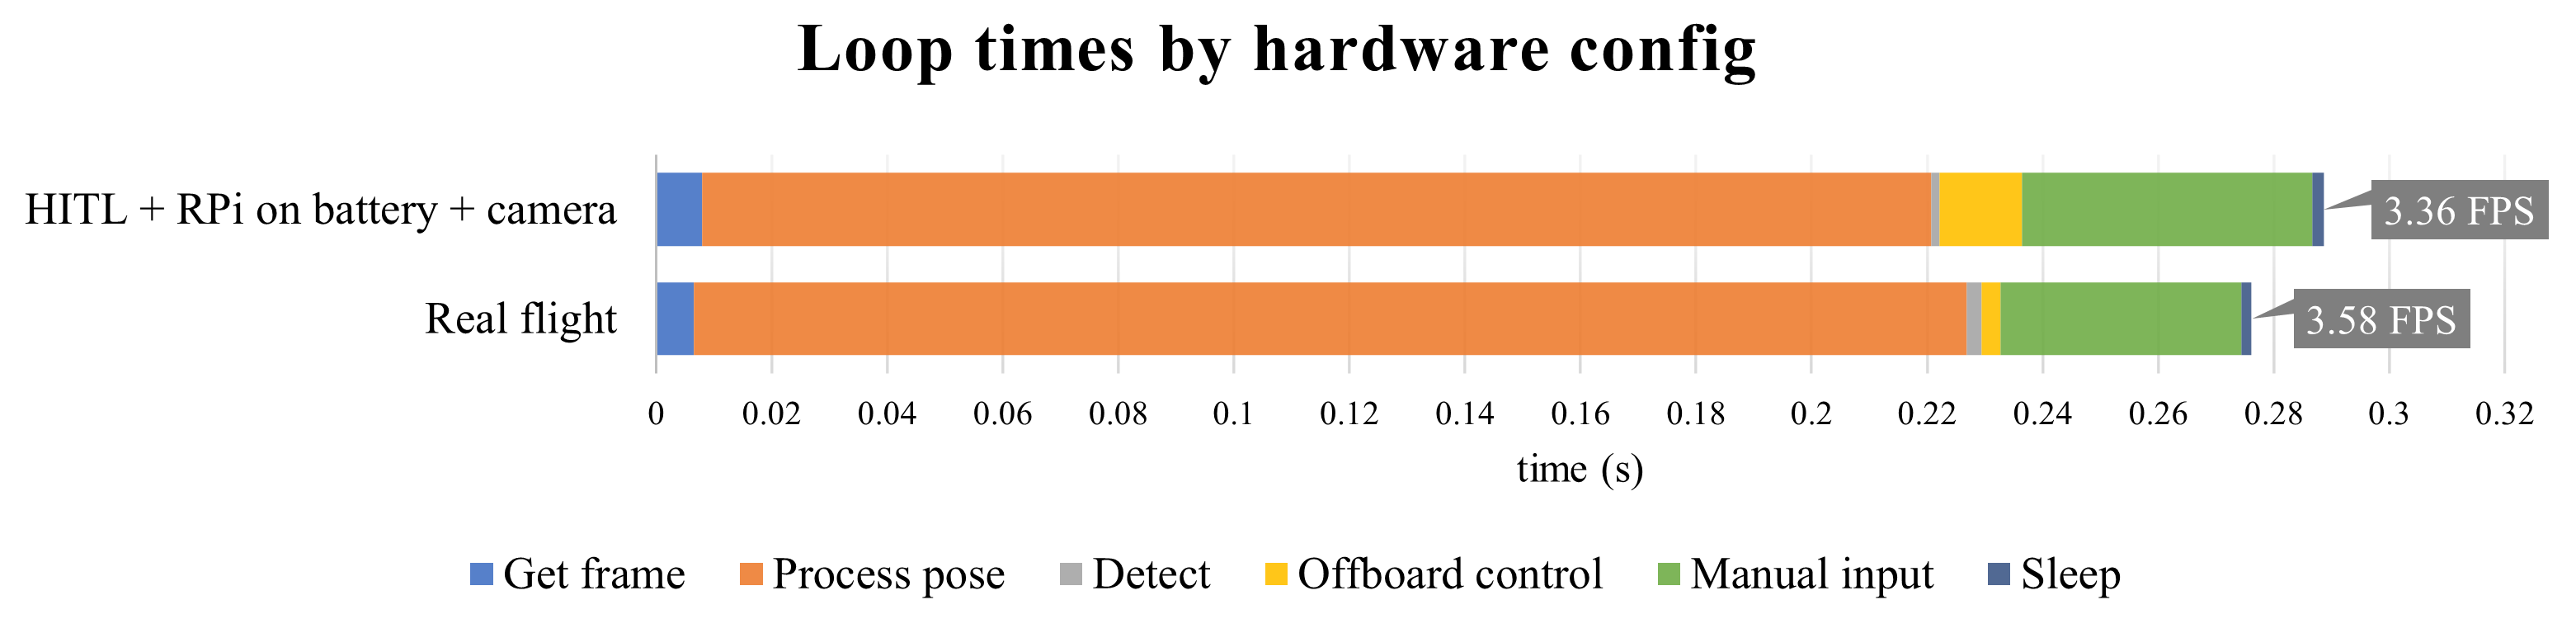
\includegraphics[width=\textwidth, keepaspectratio]{img/perf-hitl-flight.png}
  \caption{Terminal and image output of the DroneVisionControl follow solution running on the Raspberry Pi}
  \label{fig:flight-performance}
\end{figure}
